\onehalfspacing
\section{Đề số 21}
\graphicspath{{./img/}}
\begin{bt} 
    \hfill
    \begin{enumerate}[a.]
        \item Tính giá trị biểu thức $\quad \mathrm{A}=\left(2 \frac{1}{3}+3,5\right):\left(-4 \frac{1}{6}+2 \frac{1}{7}\right)+7,5$
        \item Rút gọn biểu thức $\quad B=\frac{2 \cdot 8^4 \cdot 27^2+4 \cdot 6^9}{2^7 \cdot 6^7+2^7 \cdot 40 \cdot 9^4}$
        \item Tính đa thức $\mathrm{M}$ biết rằng : $M+\left(5 x^2-2 x y\right)=6 x^2+9 x y-y^2$. Tính giá trị của $M$ khi $x, y$ thỏa mãn $(2 x-5)^{2018}+(3 y+4)^{2020} \leq 0$.
    \end{enumerate}
\loigiai{
    \begin{enumerate}
        \item $\mathrm{A}=\left(2 \frac{1}{3}+3,5\right):\left(-4 \frac{1}{6}+2 \frac{1}{7}\right)+7,5=\left(\frac{7}{3}+\frac{7}{2}\right):\left(-\frac{25}{6}+\frac{15}{7}\right)+\frac{15}{2} \\[5px]
        =\frac{35}{6}: \frac{-85}{42}+\frac{15}{2}=\frac{35}{6} \cdot \frac{-42}{85}+\frac{15}{2}=\frac{-49}{17}+\frac{15}{2}=\frac{157}{34}$
        \item $B=\frac{2 \cdot 8^4 \cdot 27^2+4 \cdot 6^9}{2^7 \cdot 6^7+2^7 \cdot 40 \cdot 9^4}=\frac{2 \cdot\left(2^3\right)^4 \cdot\left(3^3\right)^2+2^2 \cdot 2^9 \cdot 3^9}{2^7 \cdot 2^7 \cdot 3^7+2^7 \cdot 2^3 \cdot 5 \cdot\left(3^2\right)^4}=\frac{2^{13} \cdot 3^6+2^{11} \cdot 3^9}{2^{14} \cdot 3^7+2^{10} \cdot 3^8 \cdot 5}$\\[5px]
        $=\frac{2^{11} \cdot 3^6 \cdot\left(2^2+3^3\right)}{2^{10} \cdot 3^7 \cdot\left(2^4+3 \cdot 5\right)}=\frac{2}{3}$
        \item $M+\left(5 x^2-2 x y\right)=6 x^2+9 x y-y^2 \Rightarrow M=6 x^2+9 x y-y^2-\left(5 x^2-2 x y\right) \\[5px]
        \Rightarrow M=6 x^2+9 x y-y^2-5 x^2+2 x y=x^2+11 x y-y^2$\\[5px]
        Ta có : $\left\{\begin{array}{l}(2 x-5)^{2018} \geq 0 \\[5px] (3 y+4)^{2020} \geq 0\end{array} \Rightarrow(2 x-5)^{2018}+(3 y+4)^{2020} \geq 0\right.$\\[5px]
        $\text{Mà } (2 x-5)^{2018}+(3 y+4)^{2020} \leq 0 \Rightarrow(2 x-5)^{2018}+(3 y+4)^{2020}=0$\\[5px]
        $\Rightarrow\left\{\begin{array}{l}(2 x-5)^{2018}=0 \\[5px] (3 y+4)^{2020}=0\end{array} \Rightarrow\left\{\begin{array}{l}x=\frac{5}{2} \\[5px] y=-\frac{4}{3}\end{array}\right.\right.$. Thay vào ta được:\\[5px]
        $M=\left(\frac{5}{2}\right)^2+11 \cdot \frac{5}{2} \cdot\left(-\frac{4}{3}\right)-\left(\frac{-4}{3}\right)^2=\frac{25}{4}-\frac{110}{3}-\frac{16}{9}=\frac{-1159}{36}$
    \end{enumerate}
}
\end{bt}

\begin{bt}
    Tìm x biết: 
	\begin{enumerate}[a.]
        \item $-\frac{15}{12} x+\frac{3}{7}=\frac{6}{5} x-\frac{1}{2}$
        \item $\frac{1}{1.3}+\frac{1}{3.5}+\frac{1}{5.7}+\ldots .+\frac{1}{(2 x-1)(2 x+1)}=\frac{49}{99}$
        \item Tìm $x, y$ nguyên biết $2 x y-x-y=2$
    \end{enumerate}
	\loigiai{
        \begin{enumerate}
            \item $-\frac{15}{12} x+\frac{3}{7}=\frac{6}{5} x-\frac{1}{2} \Leftrightarrow \frac{6}{5} x+\frac{5}{4} x=\frac{3}{7}+\frac{1}{2}$\\[5px]
            $\Leftrightarrow\left(\frac{6}{5}+\frac{5}{4}\right) x=\frac{13}{14} \Leftrightarrow \frac{49}{20} x=\frac{13}{14} \Leftrightarrow x=\frac{130}{343}$\\[5px]
            Vậy $x=\frac{130}{343}$
            \item $\frac{1}{1.3}+\frac{1}{3.5}+\frac{1}{5.7}+\ldots .+\frac{1}{(2 x-1)(2 x+1)}=\frac{49}{99}$\\[5px]
            $\Rightarrow \frac{1}{2}\left(1-\frac{1}{3}+\frac{1}{3}-\frac{1}{5}+\frac{1}{5}+\ldots \frac{1}{2 \mathrm{x}-1}-\frac{1}{2 \mathrm{x}+1}\right)=\frac{49}{99}$\\[5px]
            $\Rightarrow \frac{1}{2}\left(1-\frac{1}{2 \mathrm{x}+1}\right)=\frac{49}{99} \Rightarrow 1-\frac{1}{2 \mathrm{x}+1}=\frac{98}{99} \Rightarrow \frac{1}{2 \mathrm{x}+1}=\frac{1}{99}$\\[5px]
            $\Rightarrow 2 x+1=99 \Rightarrow 2 x=98 \Rightarrow x=49$.\\[5px] 
            Vậy $x=49$
            \item $2 x y-x-y=2 \Leftrightarrow 4 x y-2 x-2 y=4\\[5px] \Leftrightarrow 2 x(2 y-1)-2 y+1=5 \Leftrightarrow(2 y-1)(2 x-1)=5$\\[5px]
            HS xét 4 trường hợp tìm ra $(\mathrm{x}, \mathrm{y})=\{(1 ; 3) ;(3 ; 1) ;(-2 ; 0) ;(0 ;-2)\}$\\[5px]
            Vậy $(x, y)=\{(1 ; 3) ;(3 ; 1) ;(-2 ; 0) ;(0 ;-2)\}$
        \end{enumerate}
    } 
\end{bt}

\begin{bt}
    \hfill
	\begin{enumerate}[a.]
        \item Tìm hai số nguyên dương $x$ và $y$ biết rằng tổng, hiệu và tích của chúng lần lượt tỉ lệ nghịch với $35 ; 210 ; 12$.
        \item Cho $$\frac{x}{y+z+t}=\frac{y}{z+t+x}=\frac{z}{t+x+y}=\frac{t}{x+y+z}$$. Chứng minh biểu thức $P=\frac{x+y}{z+t}+\frac{y+z}{t+x}+\frac{z+t}{x+y}+\frac{t+x}{y+z}$ có giá trị nguyên.
        \item Cho $\mathrm{a}, \mathrm{b}, \mathrm{c}, \mathrm{d} \in Z$ thỏa mãn $a^3+b^3=2\left(c^3-8 \mathrm{~d}^3\right)$.Chứng minh $\mathrm{a}+\mathrm{b}+\mathrm{c}+\mathrm{d}$ chia hết cho 3
    \end{enumerate}
	\loigiai{
        \begin{enumerate}
            \item Do tổng, hiệu và tích của $x$ và y lần lượt tỉ lệ nghịch với 35; 210; 12 .\\[5px]
            Ta có $(x+y) \cdot 35=(x-y) .210=12 . x y$\\[5px]
            Từ $(\mathrm{x}+\mathrm{y}) \cdot 35=(\mathrm{x}-\mathrm{y}) \cdot 210 \Rightarrow \frac{x+y}{210}=\frac{x-y}{35} \Rightarrow \frac{x+y}{210}=\frac{x-y}{35}=\frac{2 x}{245}=\frac{2 y}{175} \\[5px]\Rightarrow \frac{x}{7}=\frac{y}{5} \Rightarrow$
            $x=\frac{7 y}{5}$ thay vào đẳng thức $(\mathrm{x}+\mathrm{y}) \cdot 35=12 . \mathrm{xy}$ ta được\\[5px]
            $\Rightarrow y^2-5 y=0 \Rightarrow y(y-5)=0 \\[5px]\Rightarrow y \in\{0 ; 5\}$ mà $y>0$ nên $y=5$\\[5px]
            Với $y=5$ thì $\mathrm{x}=7$.
            \item $\frac{x}{y+z+t}=\frac{y}{z+t+x}=\frac{z}{t+x+y}=\frac{t}{x+y+z}\\[5px] 
            \Rightarrow \frac{y+z+t}{x}=\frac{z+t+x}{y}=\frac{t+x+y}{z}=\frac{x+y+z}{t} \\[5px]
            \Rightarrow \frac{y+z+t}{x}+1=\frac{z+t+x}{y}+1=\frac{t+x+y}{z}+1=\frac{x+y+z}{t}+1 \\[5px]
            \Rightarrow \frac{x+y+z+t}{x}=\frac{z+t+x+y}{y}=\frac{t+x+y+z}{z}=\frac{x+y+z+t}{t}$\\[5px]
            Nếu $x+y+z+t=0$ thì $P=-4$\\[5px]
            Nếu $x+y+z+t \neq 0$ thì $x=y=z=t \Rightarrow P=4$\\[5px]
            Vậy P nguyên
            \item Ta có $a^3+b^3=2\left(c^3-8 \mathrm{~d}^3\right) \Leftrightarrow a^3+b^3+c^3+\mathrm{d}^3=3 c^3-15 \mathrm{~d}^3$\\[5px]
            Mà $3 c^3-15 d^3: 3$ nên $a^3+b^3+c^3+d^3: 3$ (1)\\[5px]
            Dư trong phép chia a cho 3 là $\{0 ; \pm 1\}$ suy ra dư trong phép chia $a^3$ cho 3 cũng là $\{0 ; \pm 1\}$ hay $a \equiv a^3(\bmod 3)$\\[5px]
            Tương tự ta có $b \equiv b^3(\bmod 3) ; c \equiv c^3(\bmod 3) ; d \equiv d^3(\bmod 3)$\\[5px]
            $\Rightarrow a+b+c+d \equiv a^3+b^3+c^3+d^3(\bmod 3)(2)$\\[5px] 
            $\text { Từ (1) và (2) suy ra } \mathrm{a}+\mathrm{b}+\mathrm{c}+\mathrm{d} \text { chia hết cho } 3$
        \end{enumerate}
    }
\end{bt}

\begin{bt}
    Cho tam giác $\mathrm{ABC}, \mathrm{M}$ là trung điểm của $\mathrm{BC}$. Trên tia đối của của tia $\mathrm{MA}$ lấy điểm $\mathrm{E}$ sao cho $\mathrm{ME}=\mathrm{MA}$. Chứng minh rằng:
    \begin{enumerate}[a.]
        \item $\mathrm{AC}=\mathrm{EB}$ và $\mathrm{AC} / / \mathrm{BE}$
        \item Gọi $I$ là một điểm trên $\mathrm{AC} ; \mathrm{K}$ là một điểm trên $\mathrm{EB}$ sao cho $\mathrm{AI}=\mathrm{EK}$. Chứng minh ba điểm $\mathrm{I}, \mathrm{M}, \mathrm{K}$ thẳng hàng
        \item Từ $\mathrm{E}$ kẻ $E H \perp B C(H \in B C)$. Biết $HBE=50^{\circ} ; MEB=25^{\circ}$.
        Tính $HEM$ và $BME$
    \end{enumerate}
\loigiai{
    $$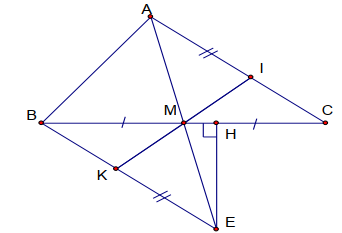
\includegraphics[width=0.5\textwidth]{21-4-lg.png}$$
    \begin{enumerate}
        \item Xét $\triangle A M C$ và $\triangle E M B$ có :\\[5px] $\mathrm{AM}=\mathrm{EM} \quad$ (gt) $A M C=E M B$ (đối đỉnh )\\[5px]
        $\mathrm{BM}=\mathrm{MC} \quad(\mathrm{gt})$\\[5px]
        $\Rightarrow \triangle A M C=\Delta E M B$ (c.g.c )\\[5px] $\Rightarrow A C=E B$ ( Hai cạnh tương ứng)\\[5px]
        Vì $\triangle A M C=\triangle E M B \Rightarrow M A C=M E B$ mà 2 góc này ở vị trí so le trong\\[5px] 
        Suy ra $A C / / B E$.
        \item Xét $\triangle A M I$ và $\triangle E M K$ có : $\mathrm{AM}=\mathrm{EM}$ (gt )
        $M A I=M E K \text { ( vì } \triangle A M C=\triangle E M B \text { ) } \\[5px]
        \mathrm{AI}=\mathrm{EK} \text { (gt) }$\\[5px]
        Nên $\triangle A M I=\Delta E M K$ ( c.g.c )\\[5px] $\Rightarrow A M I=E M K$\\[5px]
        Mà $A M I+I M E=180^{\circ}$ ( tính chất hai góc kề bù )\\[5px]
        $\Rightarrow \mathrm{EMK}+I M E=180^{\circ} \Rightarrow$ Ba điểm I; $\mathrm{M} ; \mathrm{K}$ thẳng hàng
        \item Trong tam giác vuông BHE $\left(H=90^{\circ}\right)$ có $H B E=50^{\circ}$\\[5px]
        $\Rightarrow H B E=90^{\circ}-H B E=90^{\circ}-50^{\circ}=40^{\circ} \Rightarrow H E M=H E B-M E B=40^{\circ}-25^{\circ}=15^{\circ} B M E$ là góc ngoài tại đỉnh $\mathrm{M}$ của $\triangle H E M$\\[5px]
        $\Rightarrow B M E=H E M+M H E=15^{\circ}+90^{\circ}=105^{\circ}$
    \end{enumerate}
}
\end{bt}

\begin{bt}
    Cho $B=\frac{3}{4}+\frac{8}{9}+\frac{15}{16}+\frac{24}{25}+\ldots+\frac{2499}{2500}$. Chứng tỏ $B$ không phải là số nguyên.
\loigiai{
    Ta có: $B=\frac{3}{4}+\frac{8}{9}+\frac{15}{16}+\frac{24}{25}+\ldots+\frac{2499}{2500}$\\[5px]
$B=49-\left(1-\frac{3}{4}+1-\frac{8}{9}+1-\frac{15}{16}+1-\frac{24}{25}+\ldots+1-\frac{2499}{2500}\right) \\[5px]
B=49-\left(\frac{1}{2^2}+\frac{1}{3^2}+\frac{1}{4^2}+\frac{1}{5^2}+\ldots+\frac{1}{50^2}\right)=49-\mathrm{M}$\\[5px]
Trong đó $\mathrm{M}=\left(\frac{1}{2^2}+\frac{1}{3^2}+\frac{1}{4^2}+\frac{1}{5^2}+\ldots+\frac{1}{50^2}\right)$\\[5px]
Áp dụng tính chất $\frac{1}{(n+1) n}<\frac{1}{n^2}<\frac{1}{(n-1) n}$\\[5px]
Ta có: $\left(\frac{1}{2^2}+\frac{1}{3^2}+\frac{1}{4^2}+\frac{1}{5^2}+\cdots+\frac{1}{50^2}\right)<\left(\frac{1}{2.1}+\frac{1}{3.2}+\frac{1}{4.3}+\frac{1}{5.4}+\cdots+\frac{1}{50.49}\right)$\\[5px]
$\mathrm{M}<1-\frac{1}{2}+\frac{1}{2}-\frac{1}{3}+\frac{1}{3}-\frac{1}{4}+\frac{1}{4}-\frac{1}{5}+\cdots+\frac{1}{49}-\frac{1}{50}=1-\frac{1}{50}<1$\\[5px]
Ta lại có:\\[5px]
$\mathrm{M}>\frac{1}{2.3}+\frac{1}{3.4}+\frac{1}{4.5}+\frac{1}{5.6}+\cdots+\frac{1}{50.51}=\frac{1}{2}-\frac{1}{3}+\frac{1}{3}-\frac{1}{4}+\frac{1}{4}-\frac{1}{5}+\cdots+\frac{1}{50}-\frac{1}{51} \\[5px]
\mathrm{M}>\frac{1}{2}-\frac{1}{51}=\frac{49}{101}>0$\\[5px]
Từ đó suy ra $0<M<1 \Rightarrow B=49 - M$ không phải là một số nguyên.
}
\end{bt}

